
\subsection{Ejercicio 7}

En este ejercicio debemos elegir 2 m�tricas diferentes y testear un lote de tareas \textbf{TaskBatch}, todas ellas con igual uso de CPU pero con diversas
cantidades de bloqueos. El lote de tareas utilizado es el \textit{lote3.tsk}.

Las m�tricas que elegimos fueron:
\begin{itemize}
 \item Turnaround
 \item Waiting Time 
\end{itemize}

Definidas en [Sil1] como:
\newline

\textbf{Turnaround}: Es el intervalo de tiempo entre el momento en que el proceso se carga, hasta el momento en que
el mismo termina. Es decir, es la suma de los per�odos usados en esperar datos de memoria, en estar encolado en la ``ready queue'', ejecutandose en 
la CPU, y haciendo E/S.


\textbf{Waiting Time}: Es el tiempo que un proceso se pasa encolado en la ``ready queue''.
\newline
\newline
Elegimos estas m�tricas ya que, con el Turnaround, tenemos una visi�n global de c�mo se comportan los procesos, mientras que con el Waiting Time
podemos observar c�mo un hecho m�s puntual, el tiempo que los procesos pasan encolados, impacta en el tiempo de ejecuci�n total del proceso.
\newline
\newline
Para calcular el desv�o standard utilizamos la f�rmula de [WikSD]
\newline
\newline
A continuaci�n se pueden observar los resultados de la experimentaci�n:
\newline
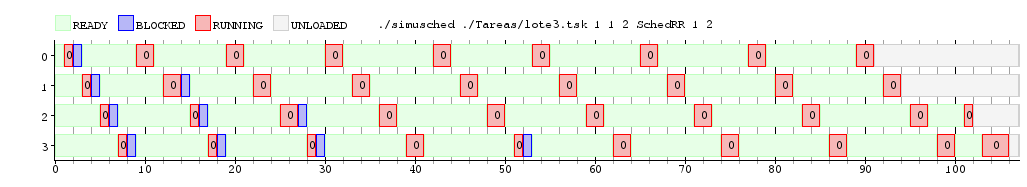
\includegraphics[width=1\textwidth]{./Graficos/ej7_1core_q2.png}
\begin{center}
 \textit{1 core, quantum = 2}.
\end{center}
~\\
\newline
Turnaround:  \hspace{7cm}  Waiting Time:

$P_{0}$: 90  \hspace{8cm}    $P_{0}$: 73

$P_{1}$: 91  \hspace{8cm}    $P_{1}$: 75

$P_{2}$: 97  \hspace{8cm}    $P_{2}$: 82

$P_{3}$: 99  \hspace{8cm}    $P_{3}$: 85


Promedio: 94,25 \hspace{6,5cm}   Promedio: 78,75


DS: 3,83         \hspace{7,7cm}    DS: 4,92
%----------------------------------------------------------------------------------------------

~\\
\newline
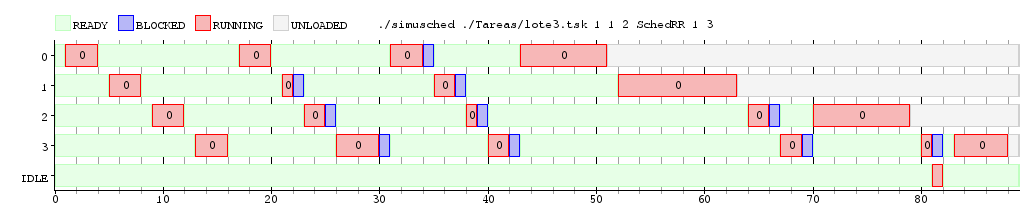
\includegraphics[width=1\textwidth]{./Graficos/ej7_1core_q3.png}
\begin{center}
 \textit{1 core, quantum = 3}.
\end{center}
~\\
\newline
Turnaround:  \hspace{7cm}  Waiting Time:

$P_{0}$: 81 \hspace{8cm}    $P_{0}$: 64

$P_{1}$: 82 \hspace{8cm}    $P_{1}$: 66

$P_{2}$: 90 \hspace{8cm}    $P_{2}$: 75

$P_{3}$: 91  \hspace{8cm}    $P_{3}$: 77


Promedio: 85,5  \hspace{6,5cm}    Promedio: 70,5


DS: 4,55        \hspace{7,6cm}    DS: 5,60
~\\
\newline


%----------------------------------------------------------------------------------------------

~\\
\newline
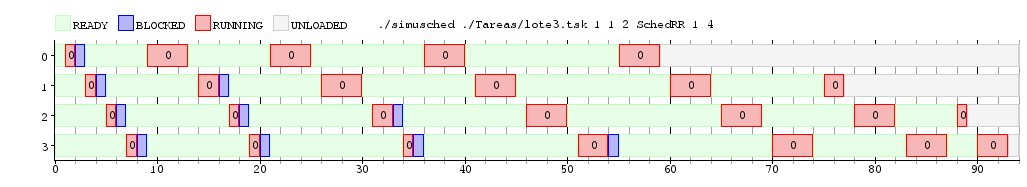
\includegraphics[width=1\textwidth]{./Graficos/ej7_1core_q4.png}
\begin{center}
 \textit{1 core, quantum = 4}.
\end{center}
~\\
\newline
Turnaround:  \hspace{7cm}  Waiting Time:

$P_{0}$: 58  \hspace{8cm}    $P_{0}$: 41

$P_{1}$: 74  \hspace{8cm}    $P_{1}$: 57

$P_{2}$: 84  \hspace{8cm}    $P_{2}$: 69

$P_{3}$: 86  \hspace{8cm}    $P_{3}$: 72


Promedio: 75,5   \hspace{6,7cm}    Promedio: 59,75


DS: 10,33         \hspace{7,5cm}    DS: 12,19
~\\
\newline




%----------------------------------------------------------------------------------------------

~\\
\newpage
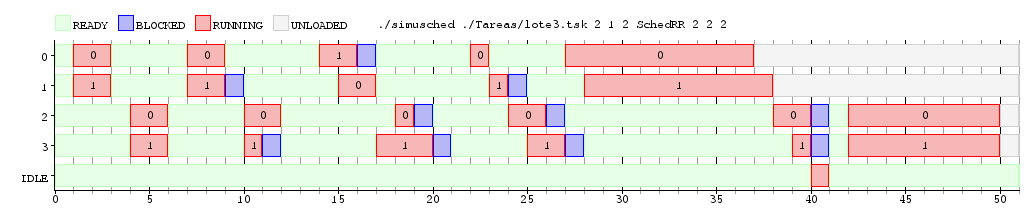
\includegraphics[width=1\textwidth]{./Graficos/ej7_2core_q2.png}
\begin{center}
 \textit{2 core, quantum = 2}.
\end{center}
~\\
\newline
Turnaround:  \hspace{7cm}  Waiting Time:

$P_{0}$: 47  \hspace{8cm}    $P_{0}$: 30

$P_{1}$: 49  \hspace{8cm}    $P_{1}$: 31

$P_{2}$: 51  \hspace{8cm}    $P_{2}$: 50

$P_{3}$: 51  \hspace{8cm}    $P_{3}$: 33


Promedio: 49,5 \hspace{6,6cm}    Promedio: 36


DS: 1,66       \hspace{7,6cm}    DS: 8,15
~\\
\newline




%----------------------------------------------------------------------------------------------

~\\
\newline
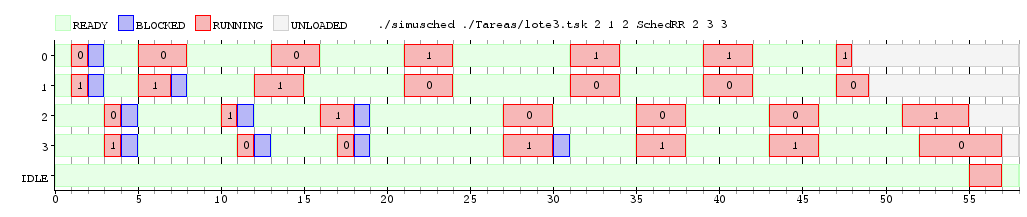
\includegraphics[width=1\textwidth]{./Graficos/ej7_2core_q3.png}
\begin{center}
 \textit{2 core, quantum = 3}.
\end{center}
~\\
\newline
Turnaround:  \hspace{7cm}  Waiting Time:

$P_{0}$: 47  \hspace{8cm}    $P_{0}$: 30

$P_{1}$: 48  \hspace{8cm}    $P_{1}$: 30

$P_{2}$: 52  \hspace{8cm}    $P_{2}$: 35

$P_{3}$: 54  \hspace{8cm}    $P_{3}$: 36


Promedio: 50,25  \hspace{6,4cm}    Promedio: 32,75


DS: 2,86         \hspace{7,6cm}    DS: 2,77
~\\
\newline




%----------------------------------------------------------------------------------------------

~\\
\newpage
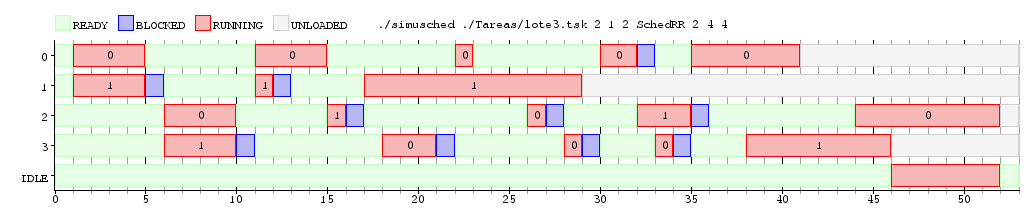
\includegraphics[width=1\textwidth]{./Graficos/ej7_2core_q4.png}
\begin{center}
 \textit{2 core, quantum = 4}.
\end{center}
~\\
\newline
Turnaround:  \hspace{7cm}  Waiting Time:

$P_{0}$: 35  \hspace{8cm}    $P_{0}$: 18

$P_{1}$: 45  \hspace{8cm}    $P_{1}$: 27

$P_{2}$: 48  \hspace{8cm}    $P_{2}$: 31

$P_{3}$: 53  \hspace{8cm}    $P_{3}$: 35


Promedio: 45,25  \hspace{6,5cm}    Promedio: 27,75


DS: 6,57        \hspace{7,6cm}    DS: 6,30
~\\
\newline


%----------------------------------------------------------------------------------------------

~\\
\newline
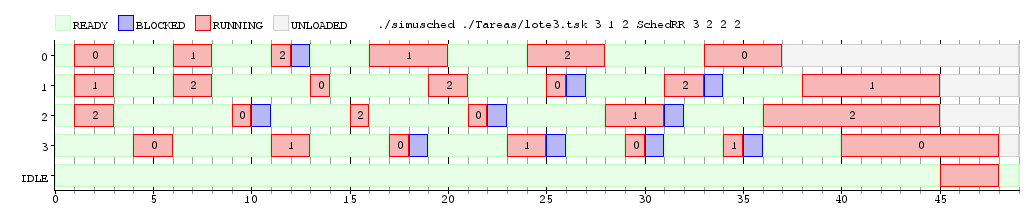
\includegraphics[width=1\textwidth]{./Graficos/ej7_3core_q2.png}
\begin{center}
 \textit{3 core, quantum = 2}.
\end{center}
~\\
\newline
Turnaround:  \hspace{7cm}  Waiting Time:

$P_{0}$: 43  \hspace{8cm}    $P_{0}$: 26

$P_{1}$: 47  \hspace{8cm}    $P_{1}$: 29

$P_{2}$: 49  \hspace{8cm}    $P_{2}$: 30

$P_{3}$: 49  \hspace{8cm}    $P_{3}$: 31


Promedio: 47  \hspace{6,9cm}    Promedio: 29


DS: 2,45          \hspace{7,6cm}    DS: 1,87
~\\
\newline



%----------------------------------------------------------------------------------------------

~\\
\newpage
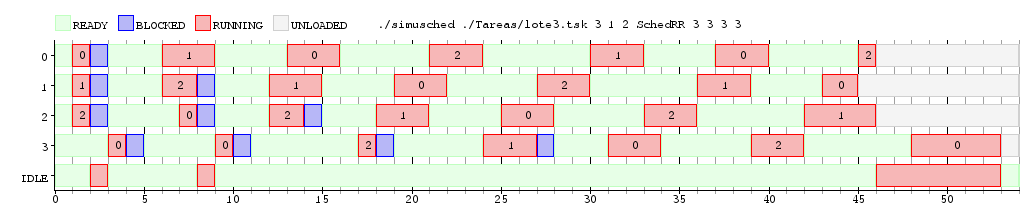
\includegraphics[width=1\textwidth]{./Graficos/ej7_3core_q3.png}
\begin{center}
 \textit{3 core, quantum = 3}.
\end{center}
~\\
\newline
Turnaround:  \hspace{7cm}  Waiting Time:

$P_{0}$: 45  \hspace{8cm}    $P_{0}$: 28

$P_{1}$: 44  \hspace{8cm}    $P_{1}$: 26

$P_{2}$: 45  \hspace{8cm}    $P_{2}$: 26

$P_{3}$: 50  \hspace{8cm}    $P_{3}$: 32


Promedio: 46   \hspace{6,9cm}    Promedio: 28


DS: 2,34        \hspace{7,6cm}    DS: 2,45
~\\
\newline



%----------------------------------------------------------------------------------------------

~\\
\newline
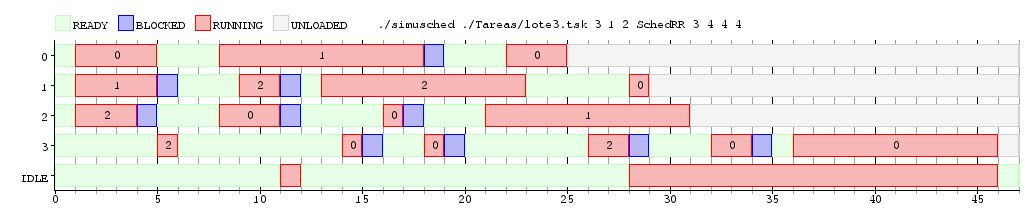
\includegraphics[width=1\textwidth]{./Graficos/ej7_3core_q4.png}
\begin{center}
 \textit{3 core, quantum = 4}.
\end{center}
~\\
\newline
Turnaround:  \hspace{7cm}  Waiting Time:

$P_{0}$: 28  \hspace{8cm}    $P_{0}$: 11

$P_{1}$: 35  \hspace{8cm}    $P_{1}$: 17

$P_{2}$: 36  \hspace{8cm}    $P_{2}$: 17

$P_{3}$: 39  \hspace{8cm}    $P_{3}$: 21


Promedio: 34,5  \hspace{6,6cm}    Promedio: 16,5


DS: 4,03          \hspace{7,6cm}    DS: 3,57 
~\\
\newline


Las conclusiones que pudimos sacar fueron las siguientes:

\begin{itemize}
 \item Dada una cantidad $i$ de cores, a medida que se aumenta el quantum, el tiempo promedio de Turnaround y Waiting Time disminuye. Esto en principio
 indicar�a que es buena idea aumentar el quantum, pero sin embargo a medida que se aumenta este, aumenta tambi�n el desv�o est�ndar, lo cual implica que los valores
 de Turnaround y Waiting Time se encuentran m�s dispersos. Esto significa que va a haber procesos que terminen relativamente r�pido mientras que otros no.
 \item Dado un mismo valor de quantum, aumentar la cantidad de cores siempre disminuye el tiempo promedio de Turnaround y Waiting Time, manteniendo o 
 reduciendo a su vez el desv�o est�ndar. Por lo tanto, obviamente, un aumento en la cantidad de cores siempre es beneficioso.
 \item El Waiting Time representa una parte muy importante del Turnaround: aproximadamente un 81\% en el caso de 1 core, 65\% con 2 cores, y 53\% con 3 cores.
 \item L�gicamente, los procesos que m�s llamadas bloqueantes realizan son los que m�s tiempo tardan en terminar. Sin embargo, en la mayor parte de los casos, 
 la diferencia en los valores de Turnaround no es demasiado significativa.
 \item El valor �ptimo del quantum para ambas m�tricas ser�a $4$, si se tolera el desv�o est�ndar asociado.
\end{itemize}
